\small
\section{はじめに}
\faTwitterSquare \,\href{https://twitter.com/hasherezade}{@hasherazade}氏が開催したMalwarebytes CrackMe 2: try another challengeのWriteUPです.CTFより問題の目的がはっきりしているため,世の中のマルウェアへ抗う手段を模索したい方,マルウェア解析者になりたい方におすすめです.

開催時は作者のGoogleDriveから入手できましたが,現在は\href{http://tinyurl.com/ybuf6z2h}{hybrid-analysis}\footnote{http://tinyurl.com/ybuf6z2h}にアップロードされています\footnote{検体の入手には認証が必要ですのでご注意を}.\faFileCodeO \,\textbf{mb\_crackme\_2.exe}は8.3MiB程度の実行ファイルです.主たる解析の流れは図\ref{fig:malware_analysis}に示した通りです.筆者はWindows10にflare-vm\footnote{マルウェア解析用にFireEye社がカスタマイズしたWindows用ツール群}を当てた環境で問題を解いています.それでは次の節から解説をはじめます.
\begin{figure}[H]
    \centering
    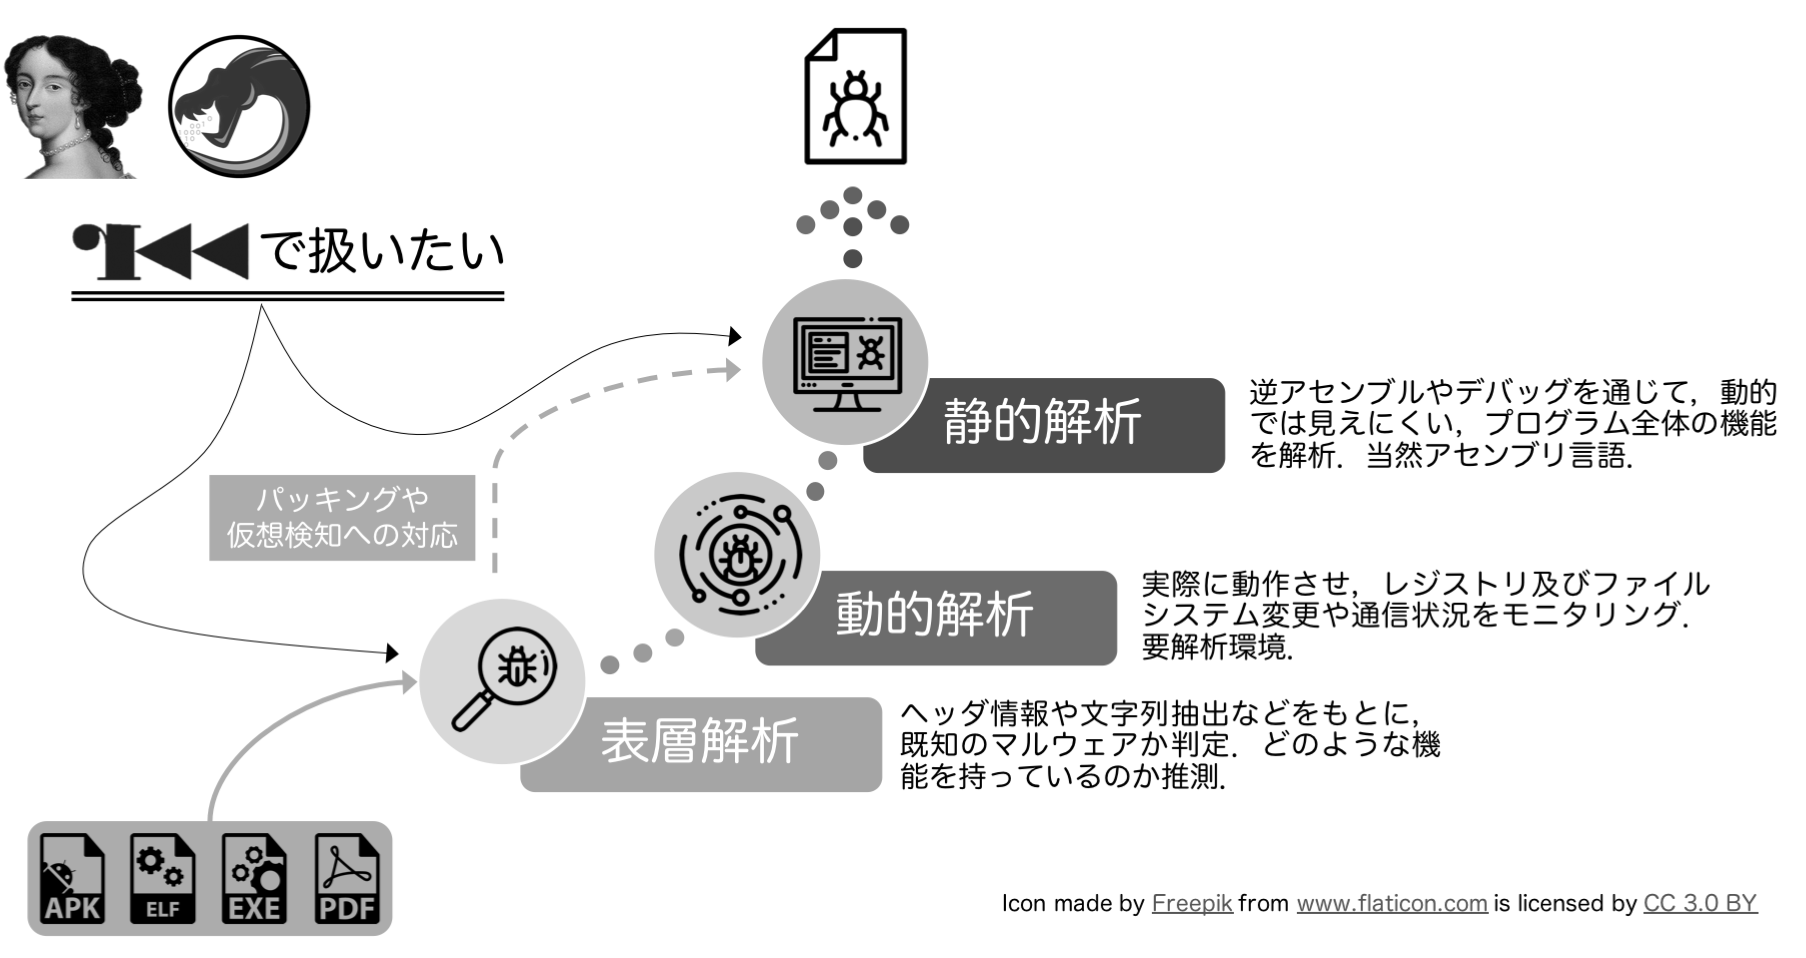
\includegraphics[width=0.85\linewidth]{./assets/takuzoo3868asset/flow_gray.png}
    \caption{マルウェア解析の概略}
    \label{fig:malware_analysis}
\end{figure}

\section{その① Login}
まず,ヘッダ情報を確認するとバイナリソースの大半は\textbf{.text}に集約されている事がわかります.一方で,リソースにはアイコン画像しか格納されていないことが確認できます.CFF Explore\footnote{ファイル識別,アドレスの変換,依存関係のスキャン,インポートされた関数を調べる際に便利なPEエディタです}を利用すると図\ref{fig:cff}のように確認できます.8.3MiBの大半が\textbf{.text}にあるということは,Hex editorを使い目的の情報を目grepするには辛すぎます.stringなどの文字列抽出ツールを使い,長い文字列を抜き出し特徴を探ってみます.

\begin{figure}[H]
    \centering
    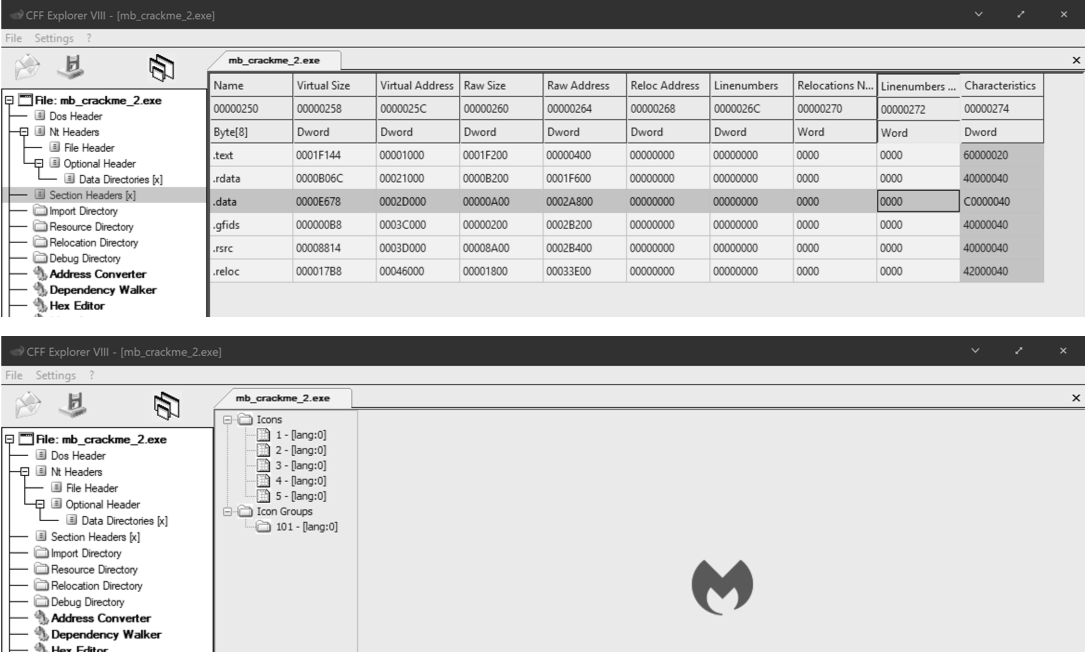
\includegraphics[width=\linewidth]{./assets/takuzoo3868asset/cff_header_gray.png}
    \caption{ヘッダ情報とリソースの確認}
    \label{fig:cff}
\end{figure}

\begin{tcolorbox}[title=文字列の抽出, sharp corners, left=2mm]\scriptsize
\begin{verbatim}
PS C:\Users\malware\Desktop\mb_2> floss.exe -n 50 -q .\mb_crackme_2.exe
Failed to get address for Py_DontWriteBytecodeFlag
Failed to get address for Py_FileSystemDefaultEncoding
Failed to get address for Py_IgnoreEnvironmentFlag
Failed to get address for PyMarshal_ReadObjectFromString
Failed to get address for PyUnicode_DecodeFSDefault
Failed to convert Wflag %s using mbstowcs (invalid multibyte string)
Failed to convert pyhome to ANSI (invalid multibyte string)
Failed to convert pypath to ANSI (invalid multibyte string)
INTERNAL ERROR: cannot create temporary directory!
 !"#$%&'()*+,-./0123456789:;<=>?@abcdefghijklmnopqrstuvwxyz[\]^_`abcdefghijklmnopqrstuvwxyz{|}~
 !"#$%&'()*+,-./0123456789:;<=>?@ABCDEFGHIJKLMNOPQRSTUVWXYZ[\]^_`ABCDEFGHIJKLMNOPQRSTUVWXYZ{|}~
_|@|P|H|X|D|T|L|\|B|R|J|Z|F|V|N|^|A|Q|I|Y|E|U|M|]|C|S|K|[|G|W|O|_
pvxHxhxXxxxDxdxTxtxLxlx\x|xBxbxRxrxJxjxZxzxFxfxVxvxNxnx^x~xAx
!P P$P P P P P P P P P P P P P P P!P%P!P!P!P!P!P!P!P!P!P!P!P!P!P!
opyi-windows-manifest-filename another.exe.manifest
\end{verbatim}
\end{tcolorbox}
flare-flossはstringsよりも強力な文字列解析ができるツールです.どうやらエラーメッセージではPythonらしきシンボルの読み出しを行っている様に思えます.よって今回はPythonスクリプトが難読化されていると目星をつけます.難読化されたPythonのスクリプトは俗にFrozen Pythonと呼ばれ,実行可能ファイルへ変換されていることがあります.このケースでは実行アプリケーションのバイトコードと依存パッケージのバイトコードが同封されている可能性が高いです.それでは確認のために,Process Explorerを使ってプログラム実行時にどのライブラリを読み込んでいるのか調査してみましょう.図\ref{fig:crackme_detail}に示したように,mb\_crackme\_2.exeはローカルにある\textbf{temp}ディレクトリからpython27.dllなどを読み出す自分のコピーを生成した様子を確認できるはずです.オリジナルのmb\_crackme\_2.exeが\textbf{\_MEI5282/temp}というディレクトリを作成し,必要なdllやpydライブラリを書き込んだのではないかと考えられます.
\begin{figure}[H]
    \centering
    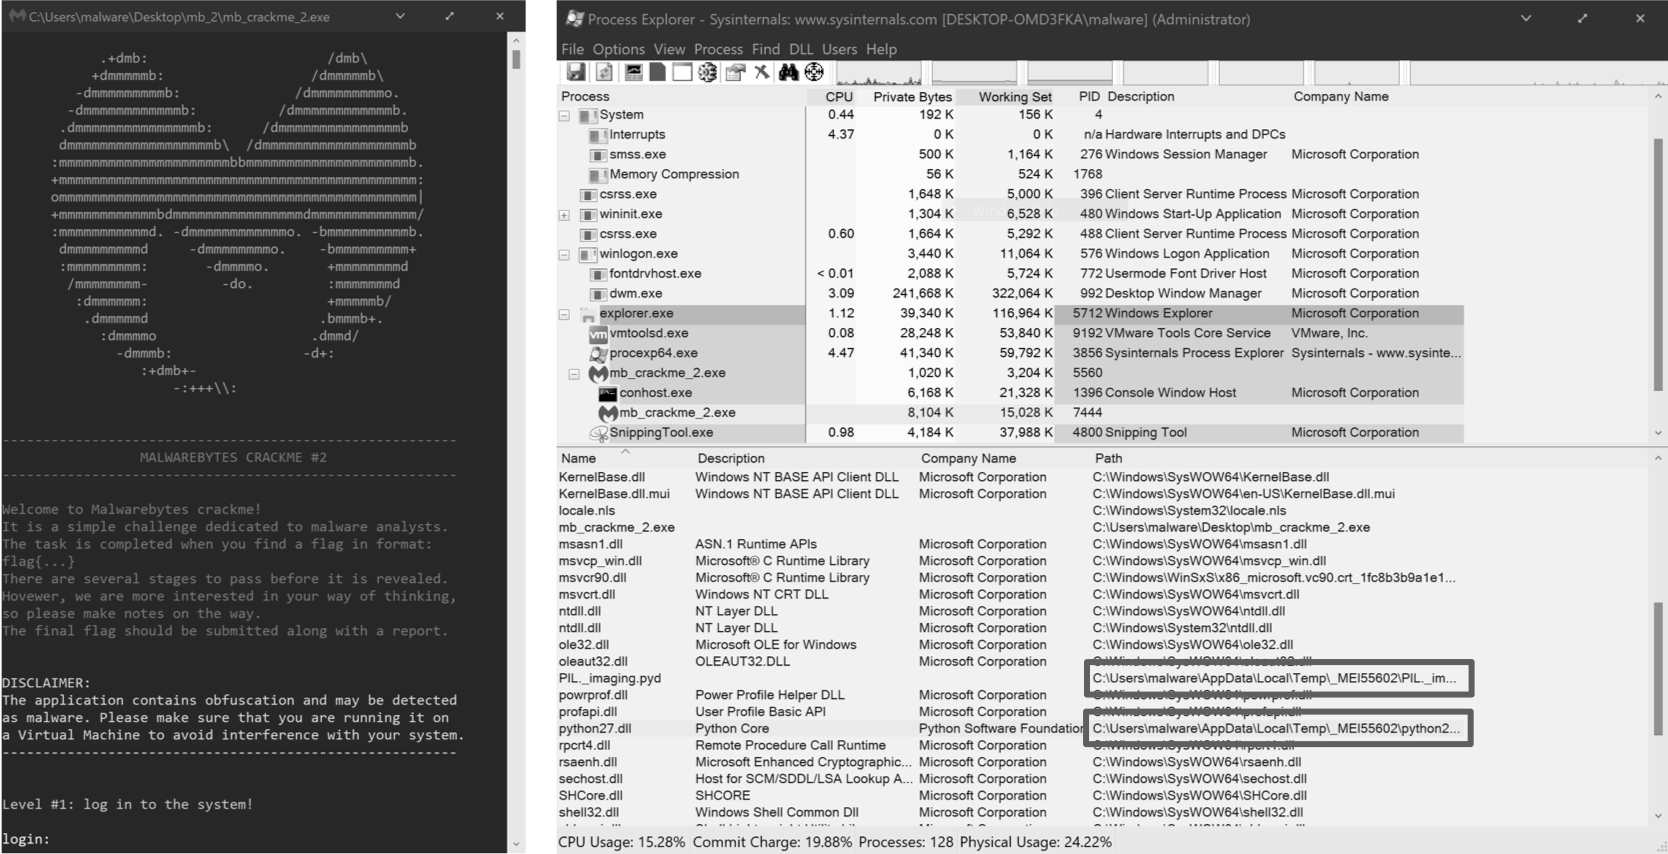
\includegraphics[width=\linewidth]{./assets/takuzoo3868asset/proc_gray.png}
    \caption{起動した様子とプロセスの監視}
    \label{fig:crackme_detail}
\end{figure}
難読化されたPythonをアンパックするために,python用のアンパッカーである\href{https://github.com/countercept/python-exe-unpacker}{python-exe-unpacker}\footnote{https://github.com/countercept/python-exe-unpacker}を使います.吐き出された中身を見ると,\faCogs \,\textbf{another}というコンパイル済みのファイルを確認できます.\href{https://github.com/rocky/python-uncompyle6}{uncompyle6}を使って逆コンパイルを試します\footnote{このツールは拡張子判定に時間がかかるため,予め.pycへ変更しておくと良いです.}が,\texttt{ImportError: Unknown magic number}となり,マジックナンバーが消えている事がわかりました.この記事\footnote{https://0xec.blogspot.com/2017/12/reversing-pyinstaller-based-ransomware.html}を参考にしたところ,PyInstallerを使ったmainスクリプトの圧縮では,時折マジックナンバーを消すことがあるので,\texttt{0x03 0xF3 0x0D 0x0A 0x00 0x00 0x00 0x00}へ書き換える必要があるとわかりました.再度逆コンパイルを試すと\faFileCodeO \,\textbf{another.py}という300行程度のソースコードを取得できました.

\begin{tcolorbox}[title=アンパック, sharp corners, left=2mm]\scriptsize
\begin{verbatim}
PS C:\Users\malware\Desktop\mb_2> .\python_exe_unpack.py -i .\mb_crackme_2.exe
[*] On Python 2.7
[*] Processing .\mb_crackme_2.exe
[*] Pyinstaller version: 2.1+
[*] This exe is packed using pyinstaller
[*] Unpacking the binary now
[*] Python version: 27
[*] Length of package: 8531014 bytes
[*] Found 931 files in CArchive
[*] Beginning extraction...please standby
[*] Found 440 files in PYZ archive
[*] Successfully extracted pyinstaller exe.
\end{verbatim}
\end{tcolorbox}

これでCrackingの準備が整いました.ログインに関連する箇所は容易に見つかります.
\begin{tcolorbox}[sharp corners, left=2mm]\scriptsize
\begin{minted}{python}
def main():
    key = stage1_login()
    if not check_if_next(key):
        return
\end{minted}
\end{tcolorbox}
\begin{tcolorbox}[sharp corners, left=2mm]\scriptsize
\begin{minted}{python}
def stage1_login():
    show_banner()
    print colorama.Style.BRIGHT + colorama.Fore.CYAN
    print 'Level #1: log in to the system!'
    print colorama.Style.RESET_ALL
    login = raw_input('login: ')
    password = getpass.getpass()
    if not (check_login(login) and check_password(password)):
        print 'Login failed. Wrong combination username/password'
        return
    PIN = raw_input('PIN: ')
    try:
        key = get_url_key(int(PIN))
    except:
        print 'Login failed. The PIN is incorrect'
        return
    else:
        if not check_key(key):
            print 'Login failed. The PIN is incorrect'
            return

    return key
\end{minted}
\end{tcolorbox}
\texttt{stage1\_login}では\texttt{username},\texttt{password},\texttt{PIN}を要求しているようです.また,これらをチェックする関数も見つかりました.ユーザー名はただの平文で\texttt{hackerman},パスワードについてはMD5でハッシュ化されていますが,オンラインにあるdecryptor toolを使えば\texttt{Password123}とわかります.PINについては少々複雑です.\texttt{get\_url\_key}にPINを渡してキーを生成し,次に\texttt{check\_key}で検証しています.Pythonの乱数生成モジュールを使ってPINをシードとした0から9の数字からなる32桁の数列キーを生成しています.検証ではmd5のハッシュを使っているようです.PINなので4桁の可能性が高いだろうなと予想して,総当たりでキーを生成しMD5ハッシュを検証することにします.
\begin{tcolorbox}[sharp corners, left=2mm]\scriptsize
\begin{minted}{python}
def check_key(key):
    my_md5 = hashlib.md5(key).hexdigest()
    if my_md5 == 'fb4b322c518e9f6a52af906e32aee955':
        return True
    return False


def check_login(login):
    if login == 'hackerman':
        return True
    return False


def check_password(password):
    my_md5 = hashlib.md5(password).hexdigest()
    if my_md5 == '42f749ade7f9e195bf475f37a44cafcb':
        return True
    return False


def get_url_key(my_seed):
    random.seed(my_seed)
    key = ''
    for i in xrange(0, 32):
        id = random.randint(0, 9)
        key += str(id)

    return key
\end{minted}
\end{tcolorbox}

\begin{tcolorbox}[title=作成したソルバーと実行結果, sharp corners, left=2mm]\scriptsize
\begin{minted}{python}
import another

for i in xrange(1000000):
    key = another.get_url_key(i)
    if another.check_key(key):
        print 'PIN: ', i
        print 'key
\end{minted}
\begin{verbatim}
PS C:\Users\malware\Desktop\mb_2> pip install --user pycrypto Pillow colorama
PS C:\Users\malware\Desktop\mb_2> python .\solve.py
PIN:  9667
key:  95104475352405197696005814181948
\end{verbatim}
\end{tcolorbox}
これでPINも\texttt{9667}とわかりました.よって,ログインは突破できました\faAngellist .
\begin{figure}[H]
    \centering
    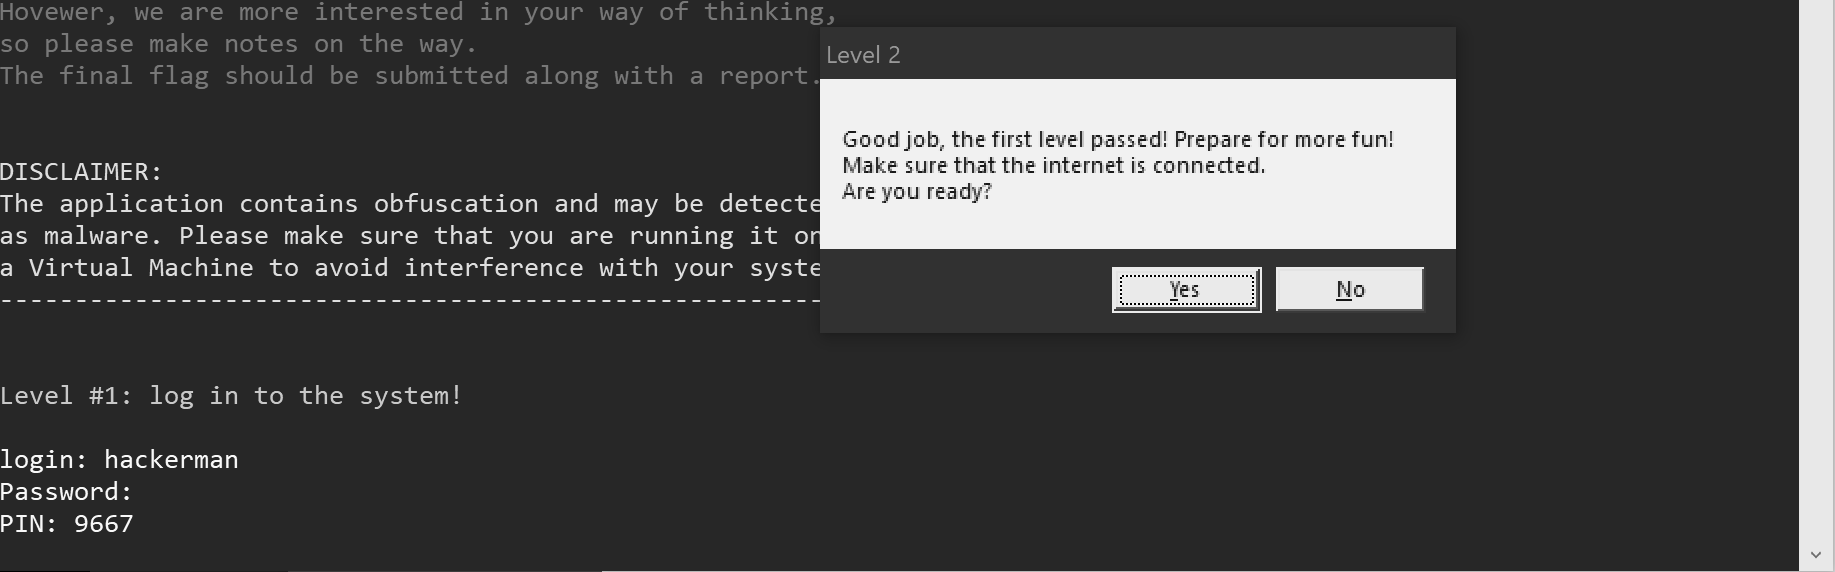
\includegraphics[width=\linewidth]{./assets/takuzoo3868asset/crack_level1_gray.png}
    \label{fig:crack_level1}
\end{figure}


\section{その② The Secret Console}
再度ソースコードを見ていきます.\texttt{check\_if\_next}でダイアログを表示し,Level2への準備ができているかどうかの確認を行っています.先程のPINを利用したキーは\texttt{decode\_and\_fetch\_url}へ渡され,AESで暗号化されたURLを復号化しリンク先から何かしらのコンテンツを取得しているように思えます.URLを確認するために\texttt{another.py}へ一行追加して実行してみました.取得できた\faFileImageO \,データを図\ref{fig:decrypt_url_data}に示します.
\begin{tcolorbox}[sharp corners, left=2mm]\scriptsize
\begin{minted}{python}
def main():
    key = stage1_login()
    if not check_if_next(key):
        return
    content = decode_and_fetch_url(key)
    if content is None:
        print 'Could not fetch the content'
        return -1
    decdata = get_encoded_data(content)
    if not is_valid_payl(decdata):
        return -3
    print colorama.Style.BRIGHT + colorama.Fore.CYAN
    print 'Level #2: Find the secret console...'
    print colorama.Style.RESET_ALL
    load_level2(decdata, len(decdata))
\end{minted}
\end{tcolorbox}
\begin{tcolorbox}[sharp corners, left=2mm]\scriptsize
\begin{minted}{python}
def decode_and_fetch_url(key):
    try:
        encrypted_url = 
'\xa6\xfa\x8fO\xba\x7f\x9d\xe2c\x81`\xf5\xd5\xf6\x07\x85\xfe[hr\xd6\x80?U\x90\x89)\xd1\xe9
\xf0<\xfe'
        aes = AESCipher(bytearray(key))
        output = aes.decrypt(encrypted_url)
        full_url = output
        print "DEBUG : URL fetched is : %s " % full_url #added from original code
        content = fetch_url(full_url)
    except:
        return

    return content
\end{minted}
\end{tcolorbox}
\begin{tcolorbox}[sharp corners, left=2mm]\scriptsize
\begin{minted}{python}
login: hackerman
Password:
PIN: 9667
DEBUG : URL fetched is : https://i.imgur.com/dTHXed7.png
\end{minted}
\end{tcolorbox}
\begin{figure}[htb]
    \centering
    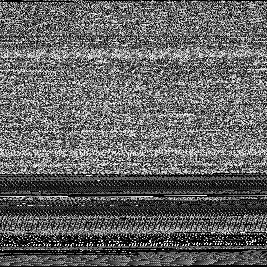
\includegraphics[width=0.4\linewidth]{./assets/takuzoo3868asset/dTHXed7_gray.png}
    \caption{プログラムが取得していた画像データ}
    \label{fig:decrypt_url_data}
\end{figure}
一見するとただのPNG形式ですが,明らかに怪しいノイズデータとなっています.無害なファイル形式を装ってコンテンツをローカルへ保存する手法はネットワークの監視をすり抜ける常套手段でもあります.今回の例であれば,監視ツールから見るとimgurからただ画像を取得したと判断されたのだと思います.特にPNG形式は可逆圧縮なのでコンテンツの隠れ蓑として優秀であると言えます\footnote{CTFで言えば意図的に情報を隠すステガノグラフィとして一大分野になっていますよね...?}.関数\texttt{get\_encoded\_data}ではPNG形式のRGB成分からバイトコードへ変換されています.また,フォーマットを解析して,バイトコードからコンテンツを展開するためにPILを使った関数は\texttt{is\_valid\_payl}でした.関数内でチェックしている23117と17744は,16進数へ変換してやるとMZやPEのマジックナンバーであることに気が付きました.つまり,この関数はデコードしたデータをPE形式などの実行可能ファイルへ変換していると推察できます.実行ファイルを抽出するために\texttt{another.py}を再度書き換えます.\texttt{main}では次に\texttt{load\_level2}へデコードしたデータを渡しています.
\begin{tcolorbox}[sharp corners, left=2mm]\scriptsize
\begin{minted}{python}
def is_valid_payl(content):
    if get_word(content) != 23117:
        return False
    next_offset = get_dword(content[60:])
    next_hdr = content[next_offset:]
    if get_dword(next_hdr) != 17744:
        return False
    return True
\end{minted}
\end{tcolorbox}
\begin{tcolorbox}[sharp corners, left=2mm]\scriptsize
\begin{minted}{python}
def load_level2(rawbytes, bytesread):
    try:
        if prepare_stage(rawbytes, bytesread):
            return True
    except:
        return False

def prepare_stage(content, content_size):
    virtual_buf = kernel_dll.VirtualAlloc(0, content_size, 12288, 64)
    if virtual_buf == 0:
        return False
    res = memmove(virtual_buf, content, content_size)
    if res == 0:
        return False
    MR = WINFUNCTYPE(c_uint)(virtual_buf + 2)
    MR()
    return True
\end{minted}
\end{tcolorbox}
ソースコードを読むと,この関数は,まずはじめに\texttt{VirtualAlloc}を使用して,コードを格納するための十分な領域を確保しています.第四引数の64は,\texttt{PAGE\_EXECUTE\_READWRITE}を意味するので読み書き可能・実行可能な権限で領域であるとわかります.対象は\texttt{memmove}関数によって書き込みが実行されるといった内容です.\texttt{prepare\_stage}へ数行追加してコンテンツのダンプファイルを取得してみましょう.
\begin{tcolorbox}[title=ダンプファイルの取得, sharp corners, left=2mm]\scriptsize
\begin{minted}{python}
def prepare_stage(content, content_size):
    with open("dumped_payload.dll", "wb") as f: # added from original code
        f.write(content[:content_size])
        print "DEBUG : File dumped in dumped_payload.dll"
    virtual_buf = kernel_dll.VirtualAlloc(0, content_size, 12288, 64)
    # ...
\end{minted}
\begin{verbatim}
PS C:\Users\malware\Desktop\mb_2> python .\another.py
Level #2: Find the secret console...

DEBUG : File dumped in dumped_payload.dll

PS C:\Users\malware\Desktop\mb_2> trid.exe .\dumped_payload.dll

TrID/32 - File Identifier v2.24 - (C) 2003-16 By M.Pontello
Definitions found:  11384
Analyzing...

Collecting data from file: .\dumped_payload.dll
 52.9% (.EXE) Win32 Executable (generic) (4508/7/1)
 23.5% (.EXE) Generic Win/DOS Executable (2002/3)
 23.5% (.EXE) DOS Executable Generic (2000/1)
\end{verbatim}
\end{tcolorbox}
ディレクトリに\faFileCodeO \,\texttt{dumped\_payload.dll}が保存され,実行形式であることを確認できたので,Ghidra\footnote{NSAが公開したGUIベースのリバースエンジニアリングツール.公式FAQによればGee-druhと発音します.IDAと違い無料でデコンパイラを使えます.まぁRetdecがありますが}を使って中身を解析していきます.Ghidraは\texttt{DLL entry point}へ自動遷移してくないので\footnote{使い始めたばかりで設定をよくわかってないため,こうすれば便利だととかあったらご教授ください},\texttt{SymbolTree}から\texttt{Export}で\texttt{Entry}を探すか,\texttt{SymbolTable}を展開して\texttt{entry}でフィルタをかけるなどして,\texttt{0x100086ac}へ移動します.ページ数の都合上省きますが,\texttt{DllMainCTRStartup}や他の関数のアドレス配置\footnote{FUN\_10001170以外の関数は,entry pointから遷移するFUN\_10008579に近いアドレス配置のため静的にリンクされた単一モジュールと推測しました}から\texttt{FUN\_10001170}であると仮定しました.
\begin{figure}[H]
    \centering
    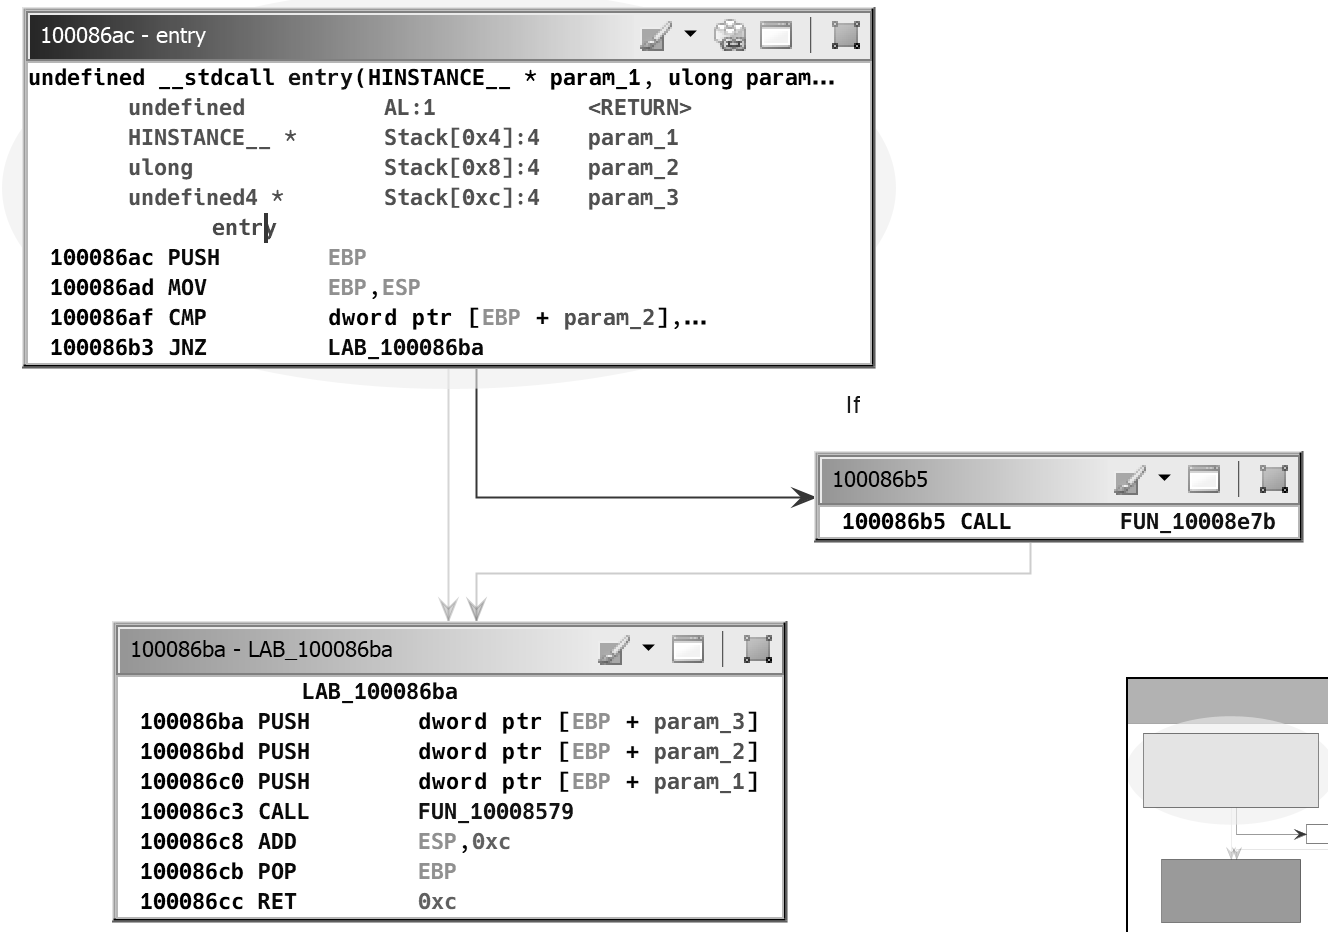
\includegraphics[width=0.7\linewidth]{./assets/takuzoo3868asset/ghidra_001_gray.png}
    \caption{DllEntryPoint function}
    \label{fig:ghdra_001}
\end{figure}
\begin{figure}[H]
    \centering
    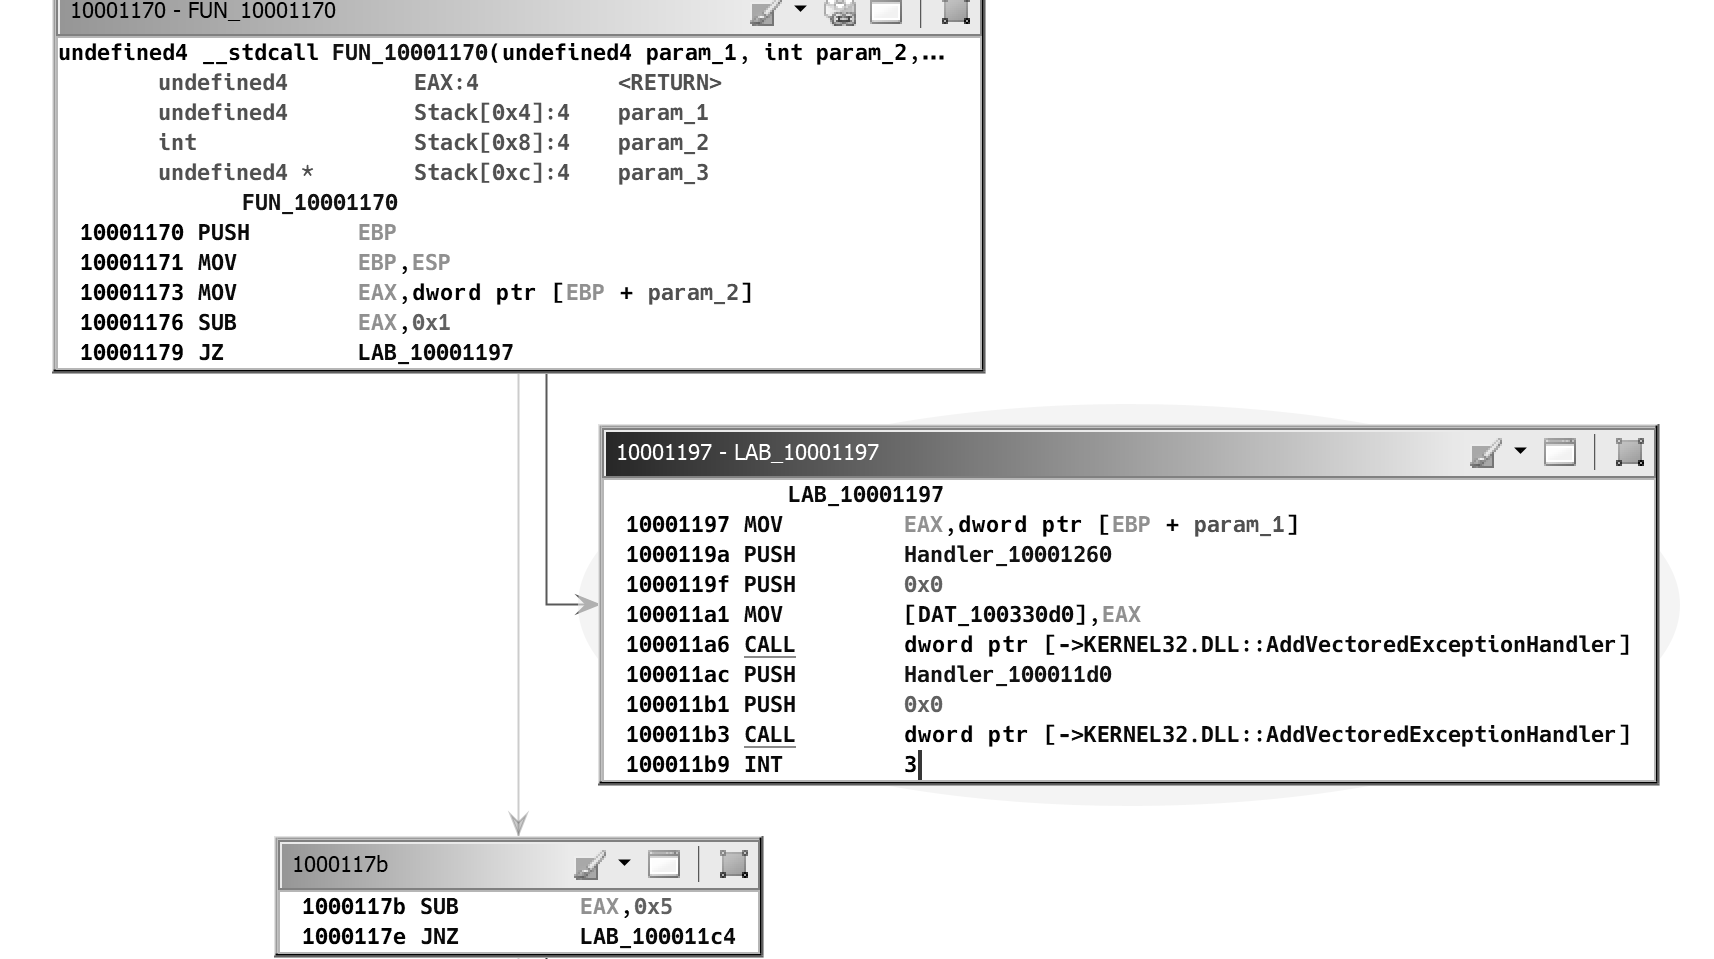
\includegraphics[width=\linewidth]{./assets/takuzoo3868asset/ghidra_002_gray.png}
    \caption{DllMain function}
    \label{fig:ghdra_002}
\end{figure}
最初のセクションでは\texttt{AddVectoredExceptionHandler}を呼び出して例外ハンドラを2つ設定しています.ここで面白い処理をしているのが\texttt{0x100011b9}にある\texttt{INT 3}です.割り込みにより自発的に例外を発生させ,例外ハンドラへ遷移するように仕掛けてあります. 解析により2つハンドラは\texttt{Handler\_10001260},\texttt{Handler\_100011d0}であると判明しています.\texttt{Handler\_10001260}では,\texttt{python27.dll}のロードを検出し,変数\texttt{mb\_chall}にプロセスIDを格納しています.\texttt{EXCEPTION\_CONTINUE\_SEARCH}で最終的には次のハンドラへ遷移します.\texttt{Handler\_100011d0}では,\texttt{python27.dll}のロードを検出し,\texttt{EIP}\footnote{Extended Instruction Pointer Register}を1ずつ或いは6ずつ増やし,プログラムを通常実行するようOSへ指示しています.\texttt{DllMain}では,先程述べた\texttt{INT 3}例外により,例外ハンドラを呼び出すことで\texttt{EIP}には\texttt{INT 3}の先頭である\texttt{0x100011B9}が格納されます.これはマルウェアにおけるアンチデバッグの一種と考えられます.ざっくり言うと,プロセスにアタッチしているデバッガは,この\texttt{INT 3}は例外ハンドラへ渡されたわけではなく,作者が意図的に設定した命令であるとみなしてスルーしてしまいます.Pythonがロードされていないと判定した場合,先程の例外ハンドラは\texttt{EIP}を1増やし,メッセージダイアログを表示する\texttt{FUN\_100010F0}へ移ります.一方で\texttt{python27.dll}がロードされている場合には,\texttt{FUN\_100010F0}をスキップして\texttt{FUN\_00010D0}を呼び出します.
\begin{figure}[H]
    \centering
    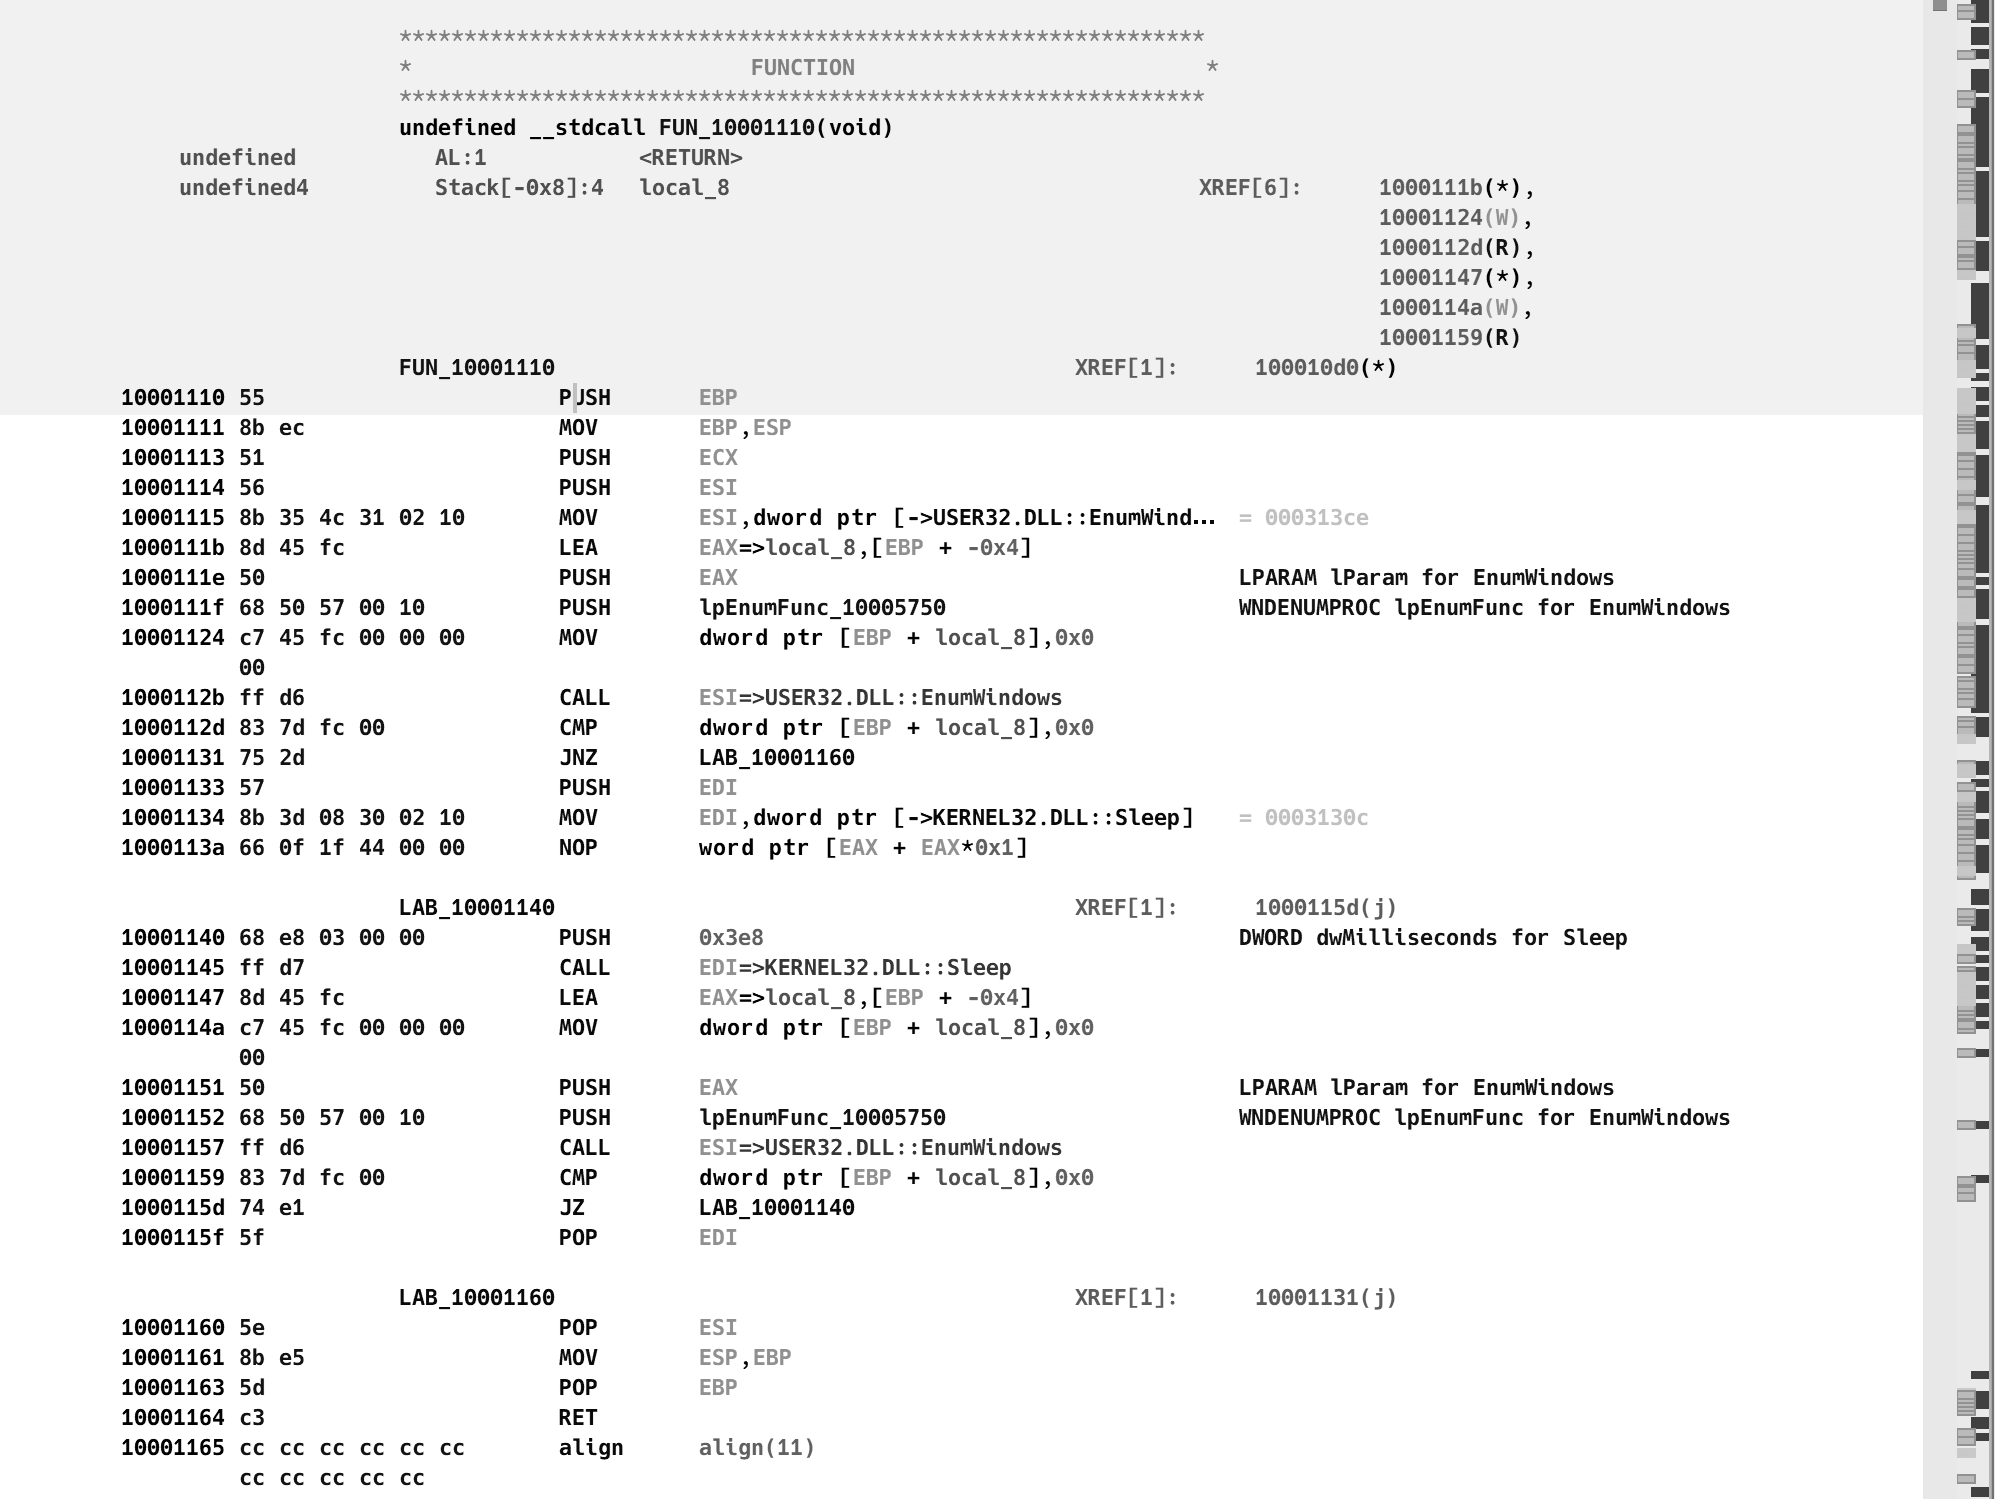
\includegraphics[width=\linewidth]{./assets/takuzoo3868asset/ghidra_003_gray.png}
    \caption{MainThread function}
    \label{fig:ghdra_003}
\end{figure}

\begin{tcolorbox}[title=例外ハンドラ箇所のclangっぽい書き方, sharp corners, left=2mm]\scriptsize
\begin{minted}{c}
LONG WINAPI Handler_10001260(struct _EXCEPTION_POINTERS *ExceptionInfo) {
   char Value[0x104];
   memset(Value, 0, sizeof(Value));
   if (GetModuleHandle("python27.dll") != 0) {
       _itoa_s(GetCurrentProcessId(), Value, sizeof(Value), 10);
   }
   SetEnvironmentVariable("mb_chall", Value);
   return EXCEPTION_CONTINUE_SEARCH;  // return 0
}
LONG WINAPI Handler_100011d0(struct _EXCEPTION_POINTERS *ExceptionInfo) {
    char Buffer[0x104];
    memset(Buffer, 0, sizeof(Buffer));
    PCONTEXT pctx = ExceptionInfo->ContextRecord;  // ebx
    DWORD delta = 1;                               // edi
    if (GetEnvironmentVariable("mb_chall", Buffer, sizeof(Buffer))) {
        if (sub_1000E409(Buffer) == GetCurrentProcessId())   // probably atoi()
            delta = 6;
    }
    pctx->Eip += delta;                  // EIP is at offset 0xB8 of CONTEXT
    return EXCEPTION_CONTINUE_EXECUTION; // return -1
}
\end{minted}
\end{tcolorbox}
では\texttt{FUN\_00010D0}の中身を追っていきます.\texttt{FUN\_00059d0}で\texttt{CreateThread}を呼び出してバックグラウンドスレッドを開始しています.その後に,\texttt{WaitForSingleObject}を使って,子スレッドの完了まで待機状態になる様です.スレッドの開始点は\texttt{push FUN\_10001110}でしょう.これも推測ですが.IDAを使っていた人は\texttt{StartAddress}へ変換されていたので合っていると思います.コールバック関数である\texttt{lpEnumFunc\_10005750}にて起動中のウィンドウを列挙し,\texttt{dwMilliseconds}に設定されている間隔で監視を繰り返します.起動しているウィンドウのタイトルは\texttt{WM\_GETTEXT hWnd}へ渡され,結果は\texttt{lParam}へスタックされます.以降解析を進めると\texttt{LAB\_10005823}付近から\texttt{Notepad}や\texttt{secret\_console}など特徴的な文字列が出現します\footnote{通常であれば文字列検索で先に見つかるかと思いますが,Main関数から大まかな仕組みをたどるために敢えて解説では後の方になりました}.\texttt{WM\_SETTEXT}を渡した\texttt{SendMessageA API}を使って,先程の文字列が両方存在する場合,ウィンドウのタイトルを\textbf{Secret Console is waiting for the commands...}書き換えます.更に\texttt{ShowWindow API}を使って書き換えたウィンドウを最前面に持ってくるといった処理をする様です.
\begin{figure}[H]
    \centering
    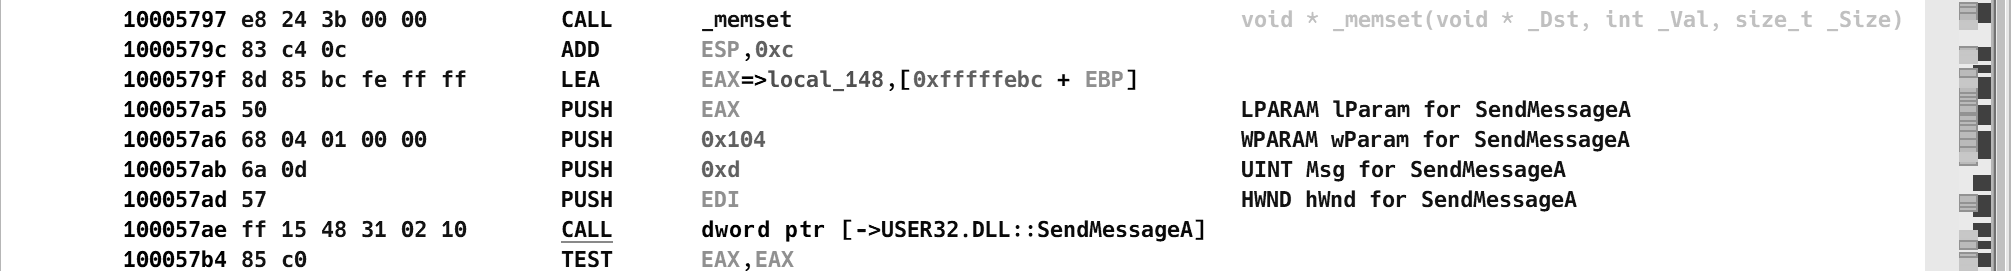
\includegraphics[width=\linewidth]{./assets/takuzoo3868asset/ghidra_004_gray.png}
    \caption{SendMessageA call in MainThread function}
    \label{fig:ghdra_004}
\end{figure}
\begin{figure}[H]
    \centering
    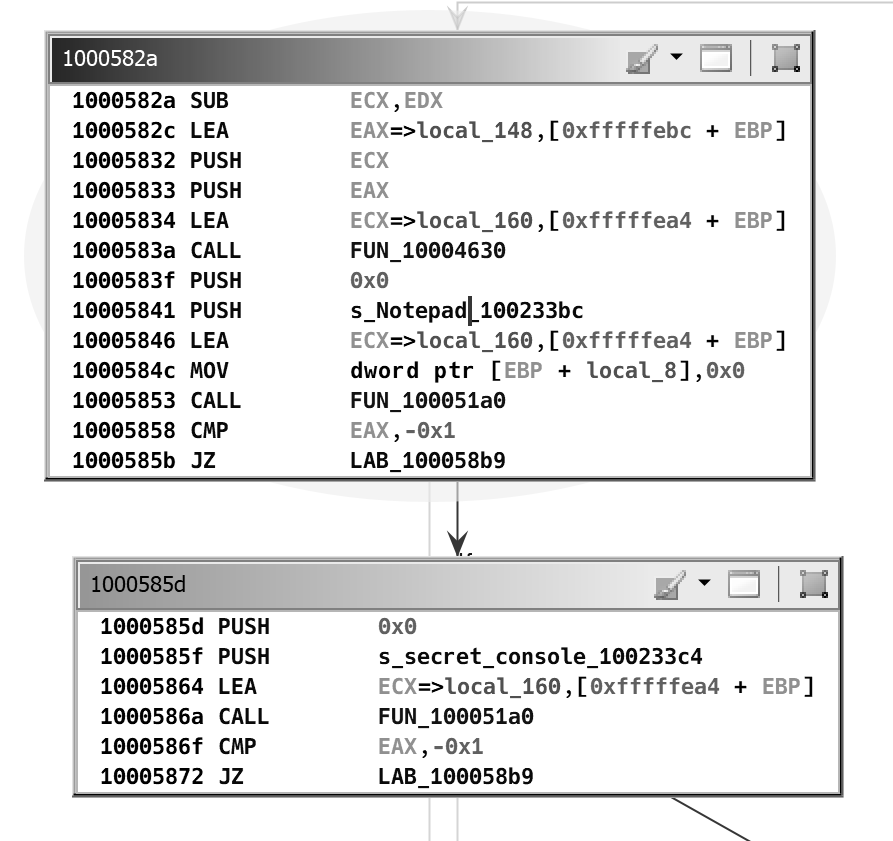
\includegraphics[width=0.5\linewidth]{./assets/takuzoo3868asset/ghidra_005_gray.png}
    \caption{"Notepad" and "secret\_console"}
    \label{fig:ghdra_005}
\end{figure}
\begin{figure}[H]
    \centering
    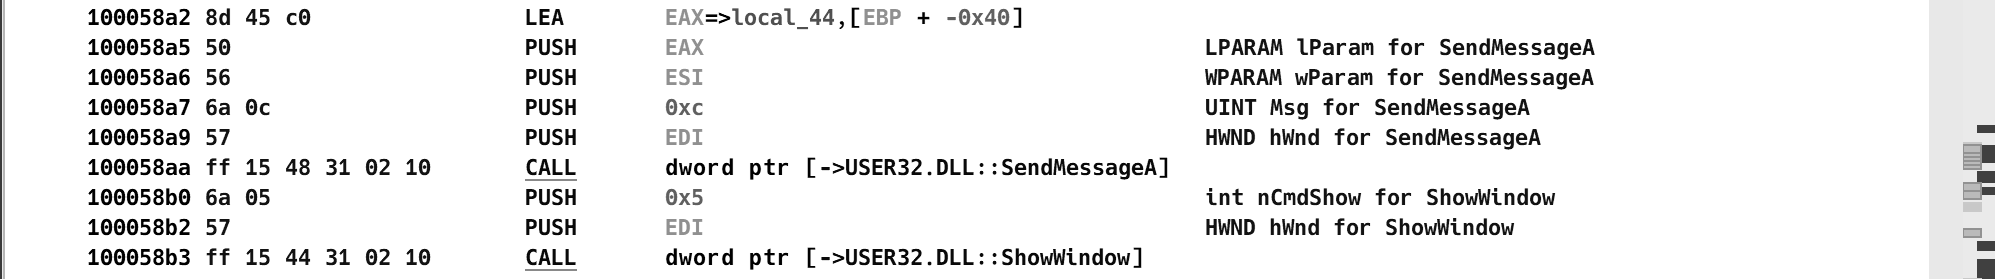
\includegraphics[width=\linewidth]{./assets/takuzoo3868asset/ghidra_006_gray.png}
    \caption{SendMessageA APIを使ったウィンドウタイトルの上書き}
    \label{fig:ghdra_006}
\end{figure}

\begin{figure}[H]
    \centering
    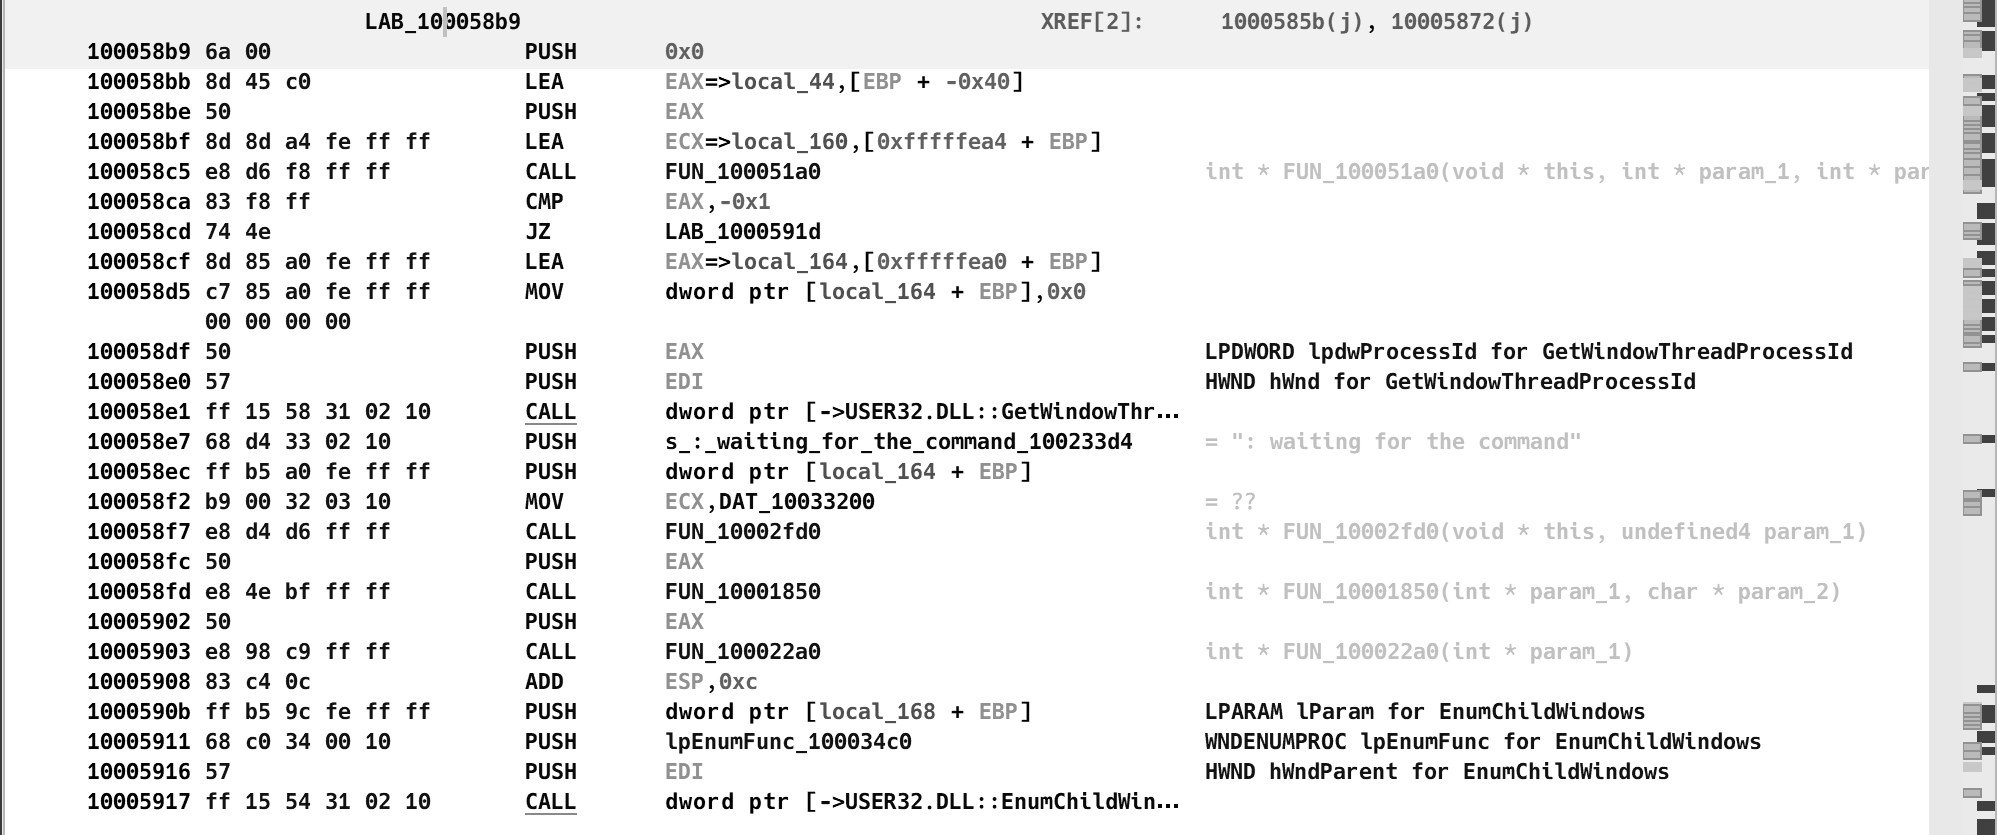
\includegraphics[width=\linewidth]{./assets/takuzoo3868asset/ghidra_007_gray.png}
    \caption{call EnumChildWindows API}
    \label{fig:ghdra_007}
\end{figure}
\begin{figure}[H]
    \centering
    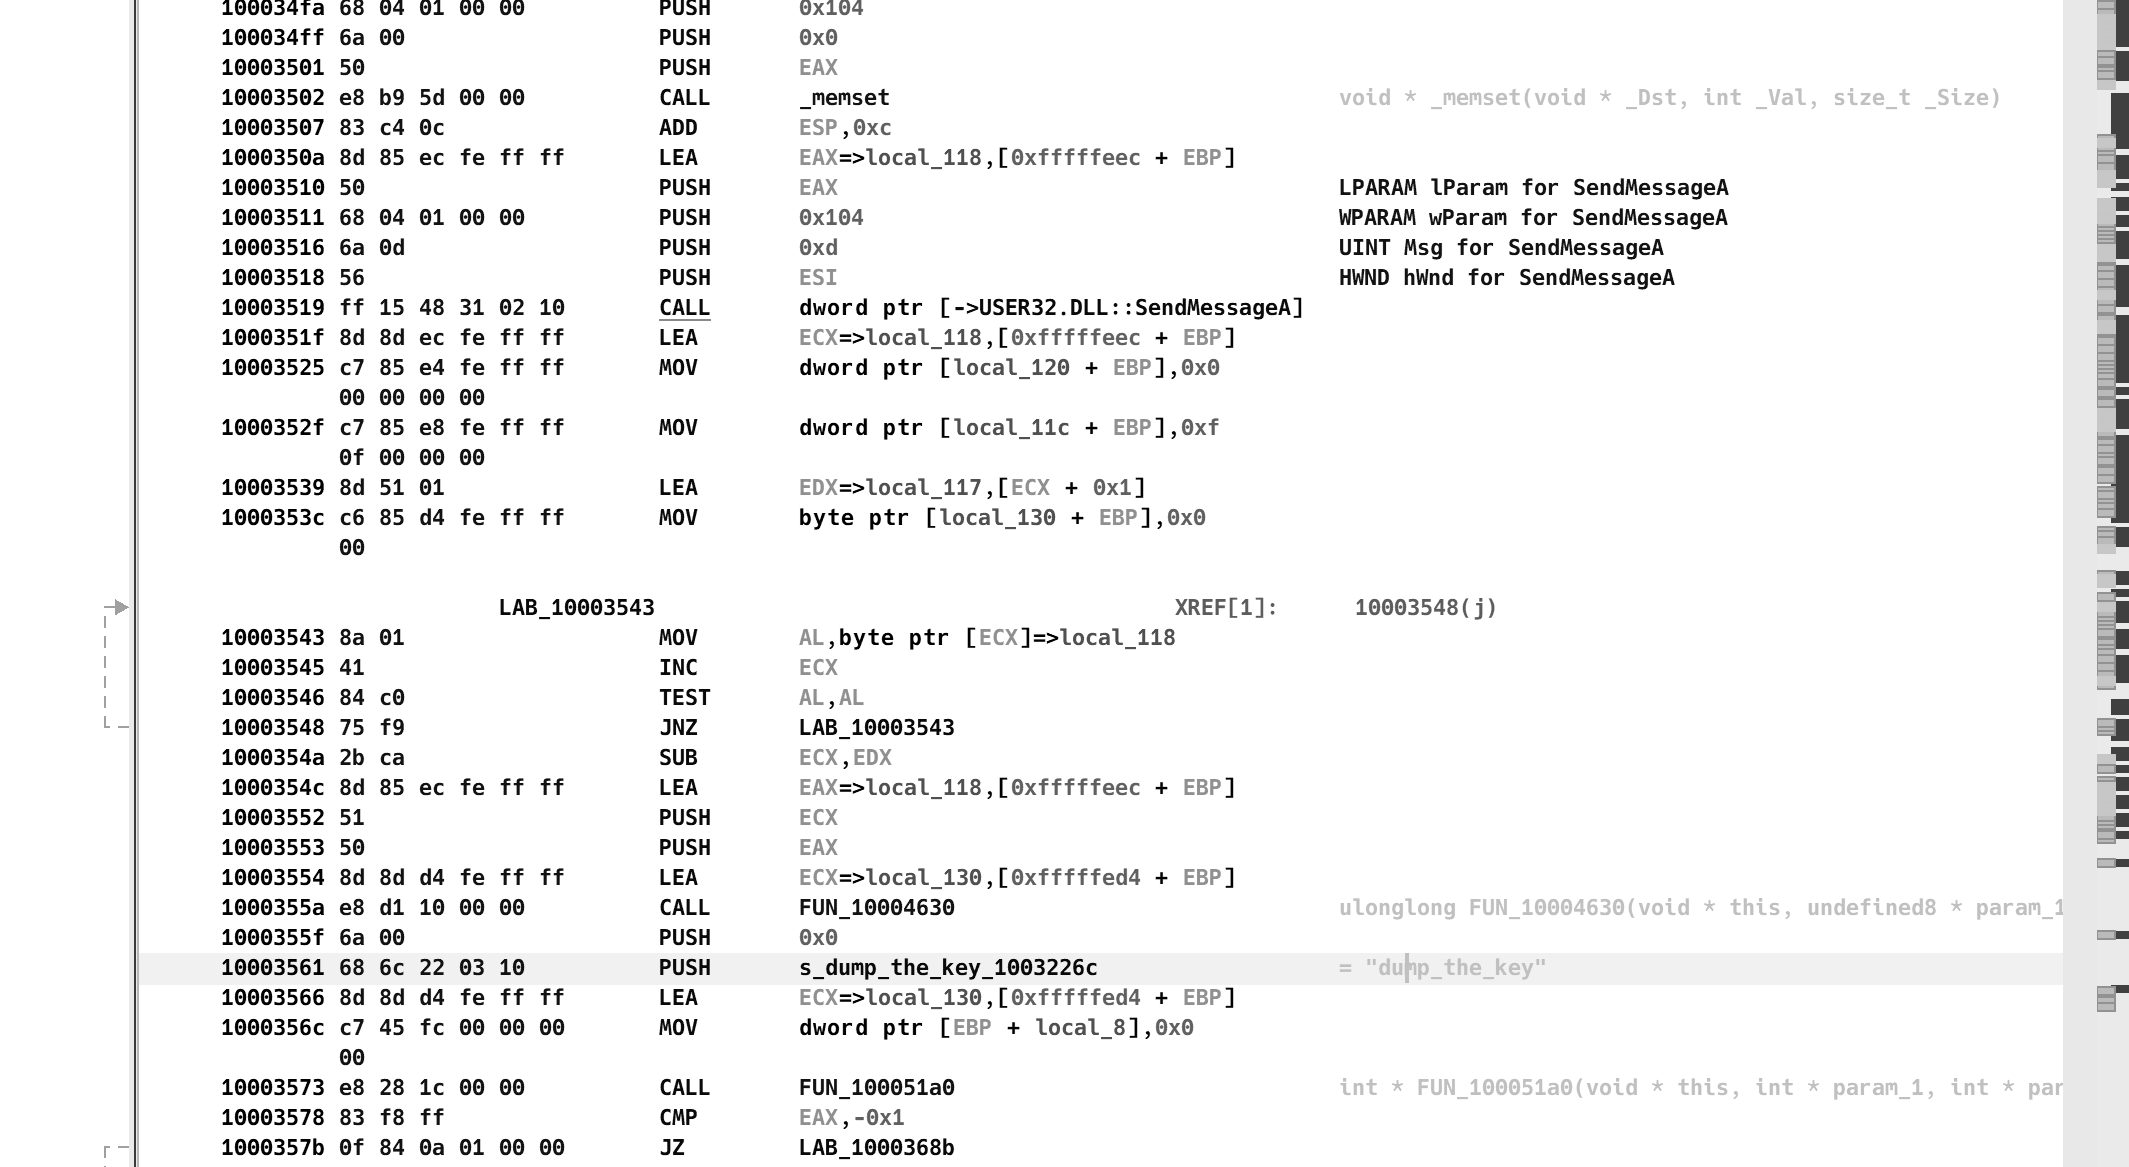
\includegraphics[width=\linewidth]{./assets/takuzoo3868asset/ghidra_008_gray.png}
    \caption{"dump\_the\_key"}
    \label{fig:ghdra_008}
\end{figure}
処理は\texttt{EnumChildWindows API}を使って子ウィンドウの列挙へと移ります.なので,次に注目すべきは\texttt{lpEnumFunc\_100034c0}内部となります.すぐに\texttt{dump\_the\_key}という怪しい文字列が見つかるはずです.周辺の処理をざっくり眺めると,\texttt{SendMessageA API}を叩いてサブウィンドウの内容を取得し,\texttt{dump\_the\_key}と合致するコンテンツを検索します.発見した場合は文字列そのものを引数として\texttt{decrypt\_buffer}を呼び出します.その後,\texttt{actxprxy.dll}がメモリにロードされ,先程復号化処理を行ったデータを\texttt{actxprxy.dll}の先頭から4096byteに書き込み,スレッド処理及びDllEntryPointも終了し,プロセス制御をmb\_crackme\_2.exeへ戻します.したがって,要点は以下のとおりです.
\begin{itemize}
  \item ウィンドウタイトルにsecret\_consoleが表示されるようなメモ帳を展開する
  \item メモ帳内部(サブウィンドウ)でdump\_the\_keyと入力
\end{itemize}
mb\_crackme\_2.exeをLevel2まで進めた上で,\texttt{secret\_console.txt}のような空ファイルをメモ帳で開き,dump\_the\_keyと入力してみます.無事突破できました\faThumbsOUp .
\begin{figure}[H]
    \centering
    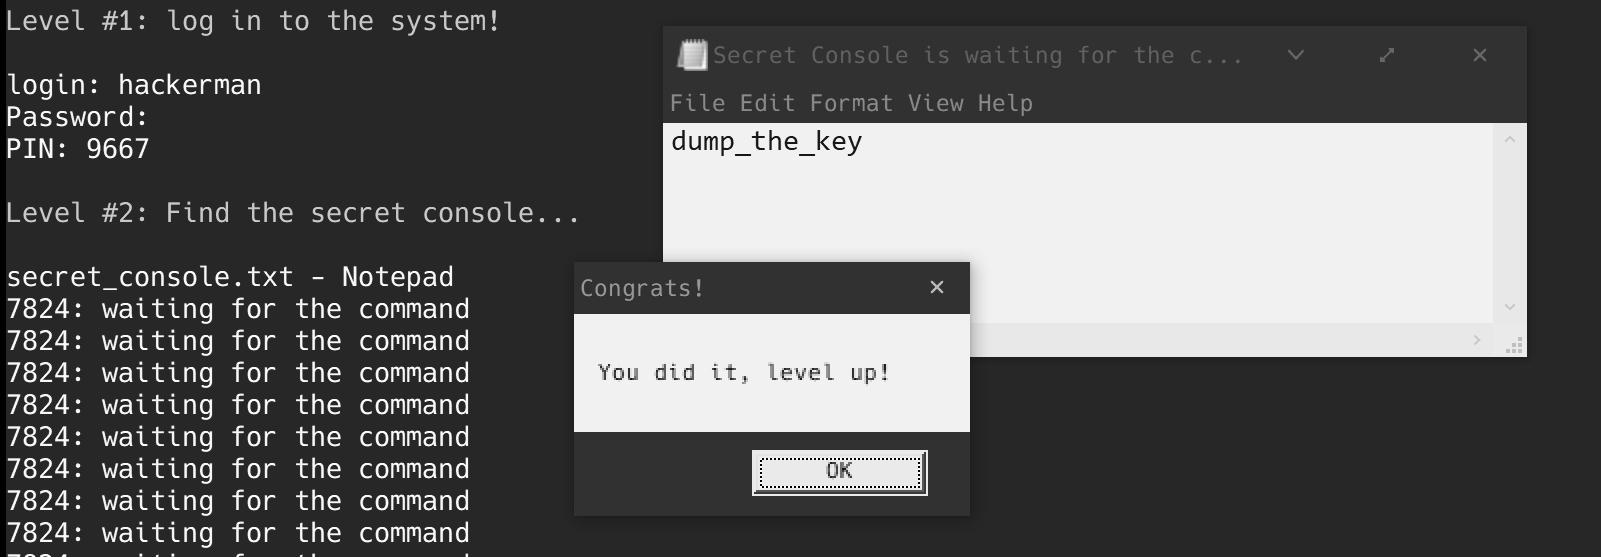
\includegraphics[width=\linewidth]{./assets/takuzoo3868asset/crack_level2_gray.png}
    \label{fig:crack_level2}
\end{figure}

\section{その③ The Color of Reverse Engineering}
次の問題は色に関係している様です.適当に入力しても駄目なので再度ソースコードを読みます.
\begin{figure}[H]
    \centering
    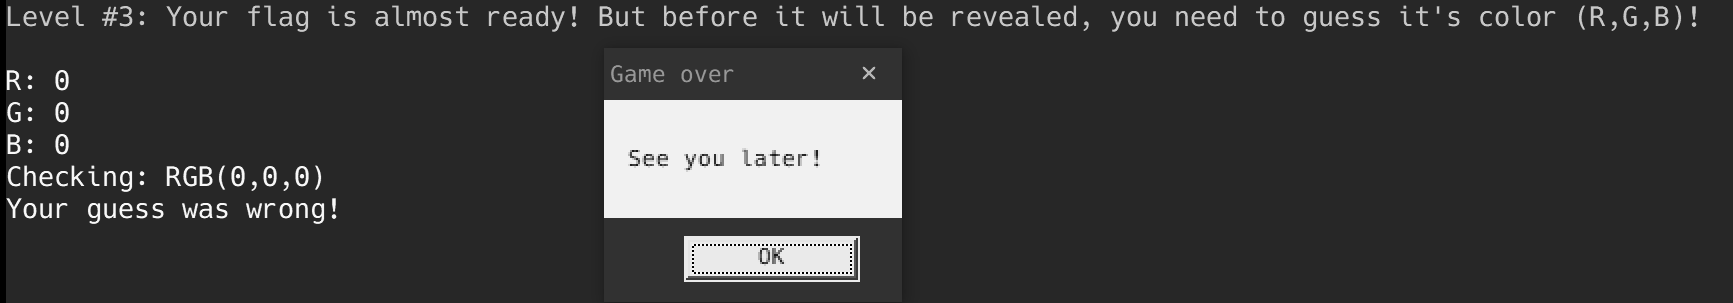
\includegraphics[width=\linewidth]{./assets/takuzoo3868asset/fail_level3_gray.png}
    \label{fig:gameover}
\end{figure}
\begin{tcolorbox}[sharp corners, left=2mm]\scriptsize
\begin{minted}{python}
def main():
    # ...
    load_level2(decdata, len(decdata))
    user32_dll.MessageBoxA(None, 'You did it, level up!', 'Congrats!', 0)
    try:
        if decode_pasted() == True:
            user32_dll.MessageBoxA(None, 
'Congratulations! Now save your flag and send it to Malwarebytes!', 'You solved it!', 0)
            return 0
        user32_dll.MessageBoxA(None, 'See you later!', 'Game over', 0)
    except:
        print 'Error decoding the flag'
\end{minted}
\end{tcolorbox}
\begin{tcolorbox}[sharp corners, left=2mm]\scriptsize
\begin{minted}{python}
def dexor_data(data, key):
    maxlen = len(data)
    keylen = len(key)
    decoded = ''
    for i in range(0, maxlen):
        val = chr(ord(data[i]) ^ ord(key[i % keylen]))
        decoded = decoded + val

    return decoded


def decode_pasted():
    my_proxy = kernel_dll.GetModuleHandleA('actxprxy.dll')
    if my_proxy is None or my_proxy == 0:
        return False
    char_sum = 0
    arr1 = my_proxy
    str = ''
    while True:
        val = get_char(arr1)
        if val == '\x00':
            break
        char_sum += ord(val)
        str = str + val
        arr1 += 1

    print char_sum
    if char_sum != 52937:
        return False
    colors = level3_colors()
    if colors is None:
        return False
    val_arr = zlib.decompress(base64.b64decode(str))
    final_arr = dexor_data(val_arr, colors)
    try:
        exec final_arr
    except:
        print 'Your guess was wrong!'
        return False

    return True
\end{minted}
\end{tcolorbox}
\texttt{main}で呼び出している\texttt{decode\_pasted}に着目すると,Level2で最後に\faCog \,\texttt{actxprxy.dll}を使い復号化したバッファを読み込んでいる様です.
\begin{enumerate}
  \item base64で復号化
  \item zlibでデータを解凍
  \item ユーザーの入力したRGB値とXOR
  \item exec関数の使用
\end{enumerate}
大まかな流れは把握できたので,\texttt{final\_arr}の中身を探します.Level2まで進めた状態でx32dbgへアタッチします\footnote{PIDがわからない場合はprocexpなどを使って調べます}.その状態でメモリマップを確認すると上書きされた\texttt{actxprxy.dll}が見つかるのでダンプします.HexEditorなどで確認すると図\ref{fig:debug_dll}のようなデータを確認できました.pythonを使ってダンプしたバイナリファイルをよしなに変換すると復号化できてしまいました.
\begin{figure}[H]
    \centering
    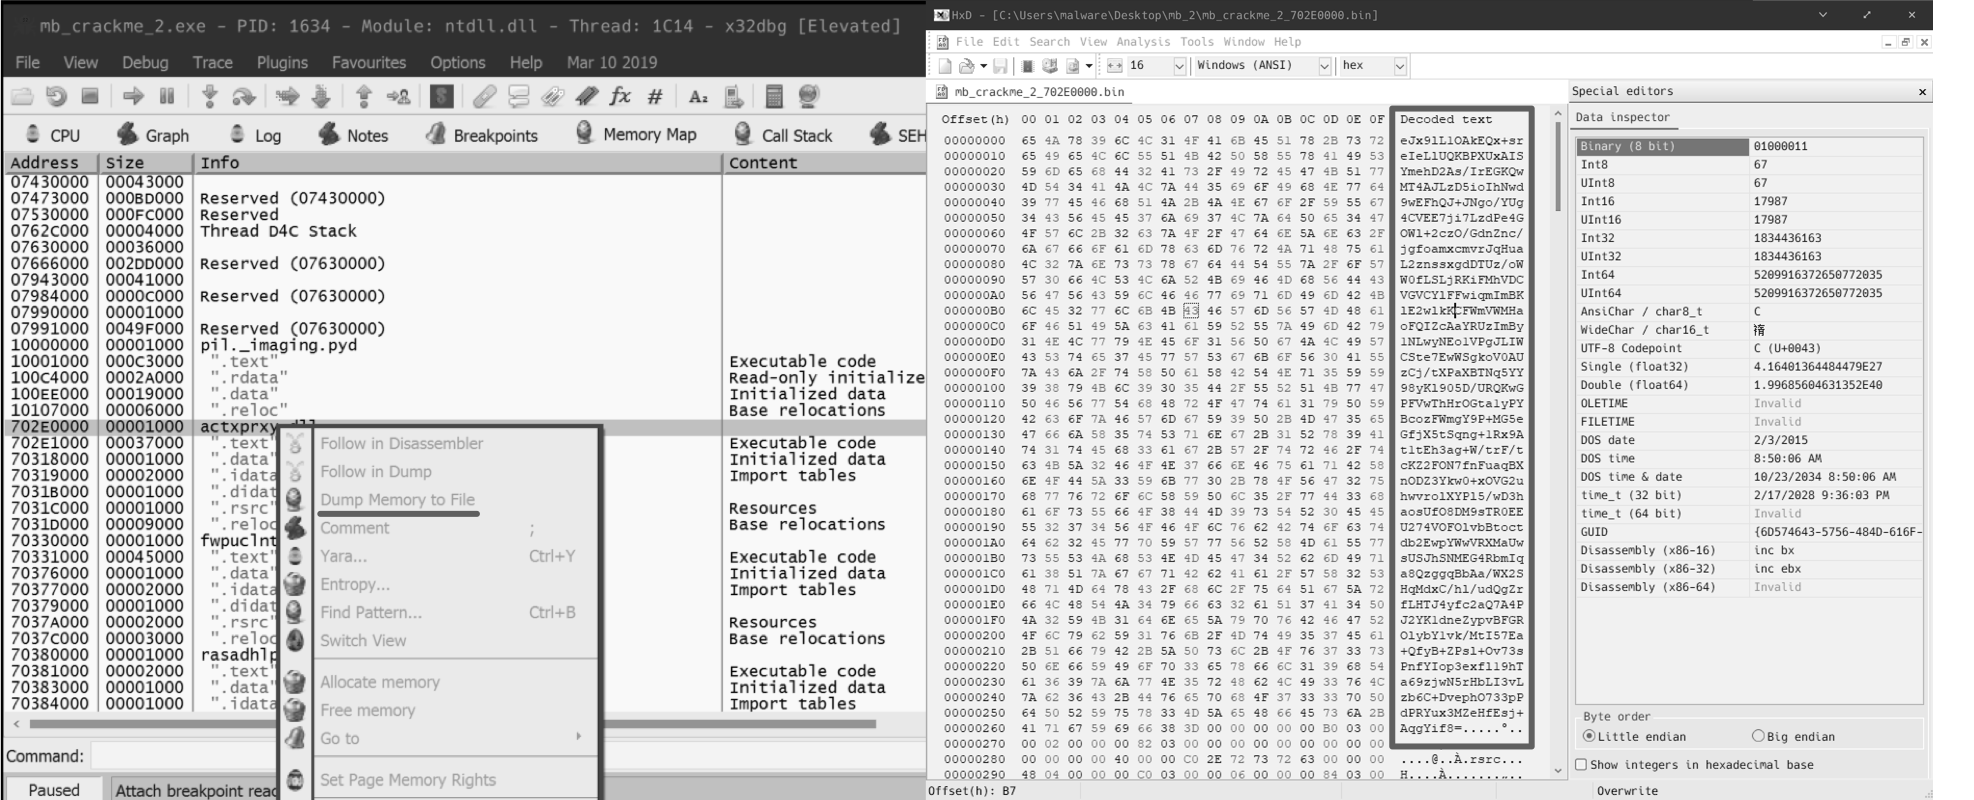
\includegraphics[width=\linewidth]{./assets/takuzoo3868asset/attach_mb_gray.png}
    \caption{ダンプしたactxprxy.dllの中身}
    \label{fig:debug_dll}
\end{figure}
\begin{tcolorbox}[title=XORを使ったデコード, sharp corners, left=2mm]\scriptsize
\begin{verbatim}
>>> import zlib
>>> from Crypto.Cipher import XOR
>>> crypted = zlib.decompress(open('702E0000.bin', 'rt').read().decode('base64'))
>>> len(crypted)
1134
>>> crypted[:8].encode('hex')
'e465e6a070f2e96e'
>>> data = XOR.new('\x80\0\x80').decrypt(crypted)
>>> print data
def print_flag():
        flag_hex = ( 
            0x73, 0x75, 0x72, 0x64, 0x65, 0x61, 0x68, 0x50, 0x20, 0x2D, 0x20, 0x22,0x2E, 0x6E, 
            0x65, 0x64, 0x64, 0x69, 0x68, 0x20, 0x79, 0x6C, 0x6C, 0x75, 0x66, 0x65, 0x72, 0x61, 
            0x63, 0x20, 0x6E, 0x65, 0x65, 0x62, 0x20, 0x73, 0x61, 0x68, 0x20, 0x74, 0x61, 0x68, 
            0x77, 0x20, 0x73, 0x65, 0x76, 0x69, 0x65, 0x63, 0x72, 0x65, 0x70, 0x20, 0x77, 0x65, 
            0x66, 0x20, 0x61, 0x20, 0x66, 0x6F, 0x20, 0x65, 0x63, 0x6E, 0x65, 0x67, 0x69, 0x6C, 
            0x6C, 0x65, 0x74, 0x6E, 0x69, 0x20, 0x65, 0x68, 0x74, 0x20, 0x3B, 0x79, 0x6E, 0x61, 
            0x6D, 0x20, 0x73, 0x65, 0x76, 0x69, 0x65, 0x63, 0x65, 0x64, 0x20, 0x65, 0x63, 0x6E, 
            0x61, 0x72, 0x61, 0x65, 0x70, 0x70, 0x61, 0x20, 0x74, 0x73, 0x72, 0x69, 0x66, 0x20, 
            0x65, 0x68, 0x74, 0x20, 0x3B, 0x6D, 0x65, 0x65, 0x73, 0x20, 0x79, 0x65, 0x68, 0x74, 
            0x20, 0x74, 0x61, 0x68, 0x77, 0x20, 0x73, 0x79, 0x61, 0x77, 0x6C, 0x61, 0x20, 0x74, 
            0x6F, 0x6E, 0x20,0x65, 0x72, 0x61, 0x20, 0x73, 0x67, 0x6E, 0x69, 0x68, 0x54, 0x22 )
        flag_str = ""
        for i in flag_hex:
                flag_str = chr(i) + flag_str
        init()
        print(Style.BRIGHT + Back.MAGENTA) + "flag{"  + flag_str + "}" + (Style.RESET_ALL)
print_flag()
\end{verbatim}
\end{tcolorbox}
flagという文字列が怪しいので,試しにスクリプトを実行するとflagを取得できました\faFlag.\textbf{flag\{"Things are not always what they seem; the first appearance deceives many; the intelligence of a few perceives what has been carefully hidden." - Phaedrus\}}プラトンのパイドロスから引用するとは洒落が効いてますね.これで正解ですがRGBが何だったのかはターミナルカラーの\texttt{MAGENTA}がヒントでした.紫色のRGBを入力すると正解みたいです.正攻法が気になります.お疲れ様でした.
\begin{figure}[H]
    \centering
    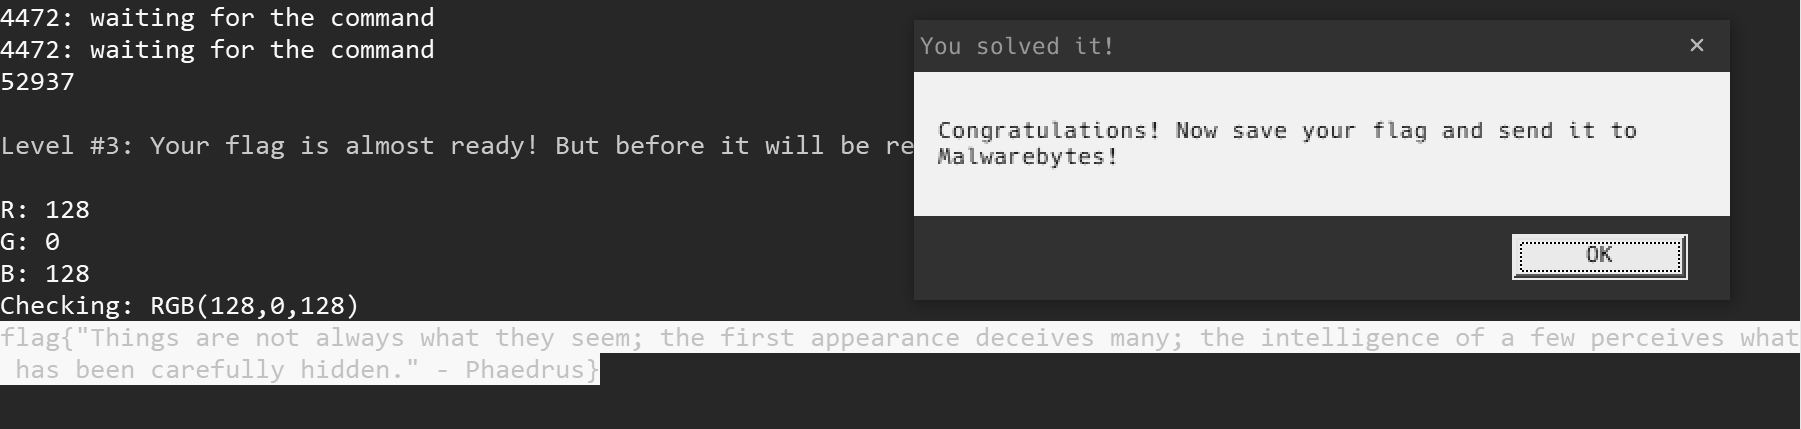
\includegraphics[width=\linewidth]{./assets/takuzoo3868asset/crack_level3_gray.png}
    \label{fig:crack_level3}
\end{figure}

\section{終わりに}
いかがだったでしょうか.いくつかのテクニックは実際にマルウェアを解析する際に役立つはずです.もし興味がお有りでしたら\href{https://crackmes.one/}{こちらのサイト}などを訪れてみてください.日夜ユーザー同士が研鑽を積んでいます.昨今,何かと逮捕案件が多くエンジニア界隈が萎縮する傾向にあります.お互いを理解するために少しでも歩み寄りが必要なのではと自分は思います.最後に作家Raymond Chandler氏の言葉をお借りして結びの言葉とします.



\textit{The law isn’t justice. It’s a very imperfect mechanism. If you press exactly the right buttons and are also lucky, justice may show up in the answer. A mechanism is all the law was ever intended to be.\\
- Raymond Chandler}
\end{document}